%projekt2 matlab
\documentclass[a4paper]{article}
\usepackage[utf8]{inputenc}
\usepackage[english,polish]{babel}
\usepackage{polski}
\usepackage[T1]{fontenc}
\frenchspacing
\usepackage{indentfirst}
\usepackage{graphicx}
\usepackage{float}

% poniższe z szablonu...
\usepackage{geometry}
\geometry{left=1in,right=1in,%
	bindingoffset=0mm, top=1in, bottom=1in}
\usepackage{amssymb, latexsym}
\usepackage{amsthm}
\usepackage{palatino}
\usepackage{array}
\usepackage{pstricks}
\usepackage{textcomp}
\usepackage{listings}

\begin{document}
	
\pagestyle{plain}
{\raggedright Alicja Obara, grupa 37 \\}
{\centering \Large Programowanie w systemie MatLab. Projekt 2\\Projekt numer 248 \\}
%\vspace{0.5cm}
\renewcommand{\thesection}{\Roman{section}}
\section{Wstęp}
%\noindent 
Obiekt regulacji opisany jest transmitancją G(s):
$$G(s)=\frac{0.1s+1.4}{(100s^2 +10s+1)(s+1)} e^{-25s}$$
Aby łatwo można było zmieniać parametry układu transmitancja została sparametryzowana do postaci:
$$G(s)=\frac{K (T_1 s+1)}{(T_2 s^2 +T_3 s+1)(T_4 s+1)} e^{-T_0 s}$$
Czas próbkowania w symulacjach $Tp=0.1$.
Odpowiedzi w punktach 1 i 2 wyznaczono na modelu (o nazwie symulacja) w programie Symulink:
\begin{figure}[H]
	\centering
	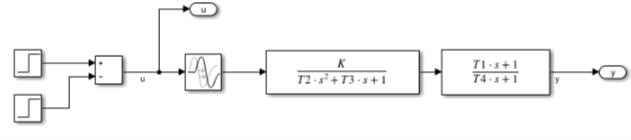
\includegraphics[width=7cm]{modelsymulacja} 
\end{figure}

\section{Wyniki}

%\renewcommand*\thesubsection{\arabic{section}}% zmiana numeracji sekcji 0.X -> X
%\setcounter{subsection}{1}
\renewcommand{\thesubsection}{\arabic{subsection}}

\subsection{Odpowiedź obiektu na wymuszenie skokowe u(t)=1(t-10).}
\begin{figure}[H]
	\centering
	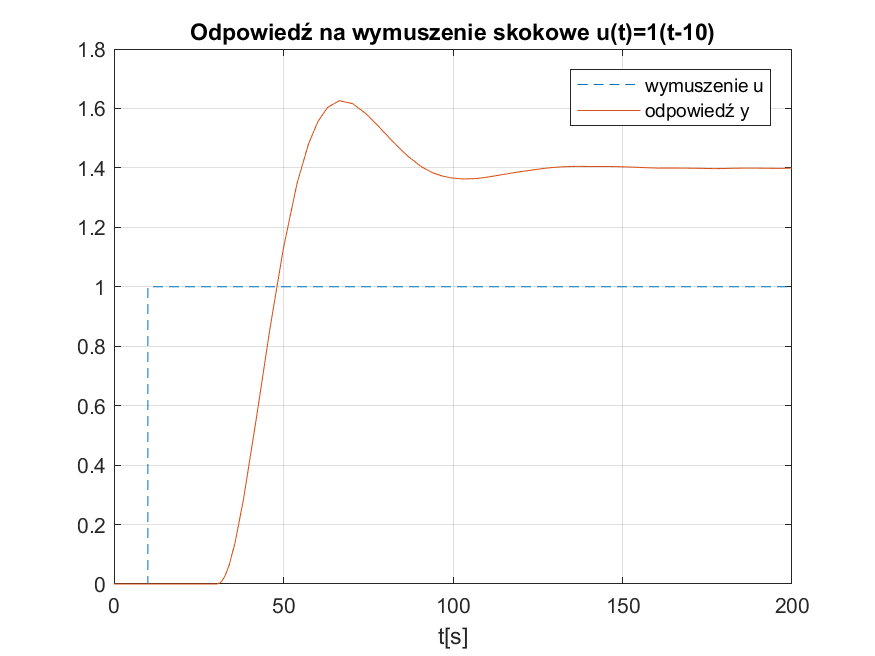
\includegraphics[width=7cm]{pkt1} 
\end{figure}

\subsection{Odpowiedź obiektu na wymuszenie pulsowe u(t)=1(t-10)-1(t-11).}
\begin{figure}[H]
	\centering
	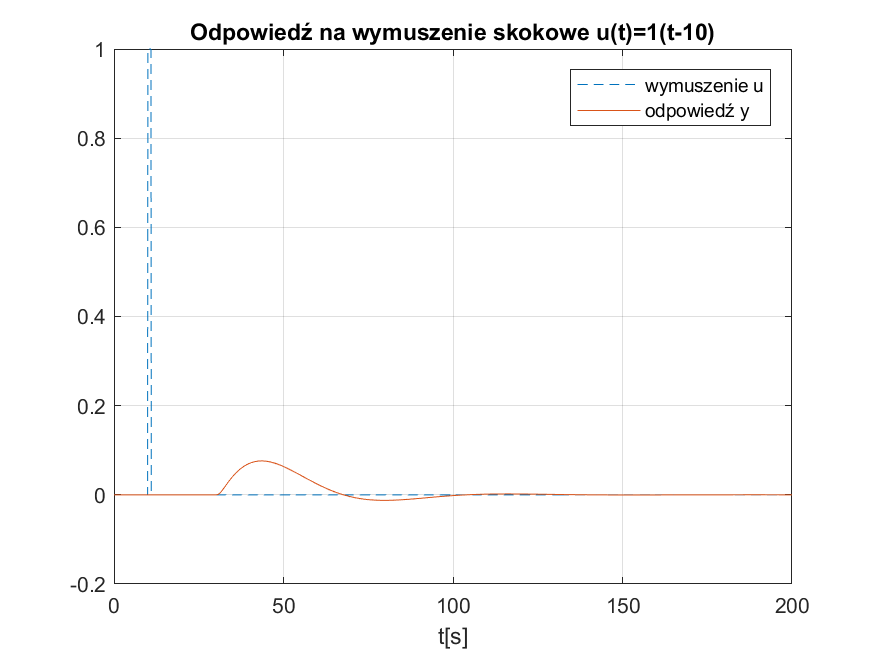
\includegraphics[width=7cm]{pkt2} 
\end{figure}

\subsection{Układ regulacji z regulatorem PID.}
Schemat modelu (o nazwie symulacjaPID) w programie Symulink:
\begin{figure}[H]
	\centering
	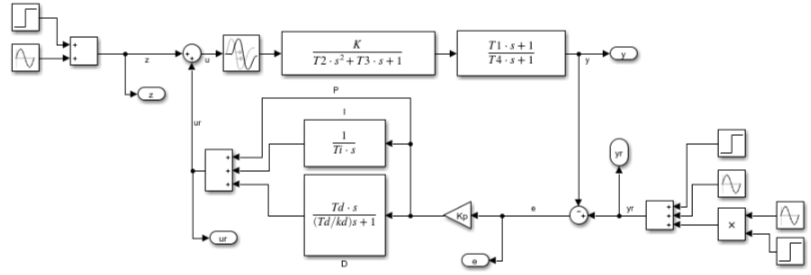
\includegraphics[width=10cm]{modelsymulacjaPID} 
\end{figure}
Zastosowano układ różniczkujący rzeczywisty o wzmocnieniu dynamicznym kd=6.
\subsection{Dobór nastaw regulatora PID.}
Zastosowano dobór nastaw metodą Zieglera-Nicholsa. Polega ona na doprowadzeniu układu tylko z akcją P regulatora do niegasnących oscylacji o okresie $T_{osc}$ przy wzmocnieniu krytycznym $k_{kryt}$.
Schemat modelu(o nazwie symulacjaZN) wykorzystanego do doboru nastaw:
\begin{figure}[H]
	\centering
	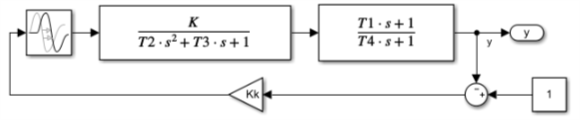
\includegraphics[width=10cm]{modelsymulacjaZN} 
\end{figure}
Niegasnące oscylacje wystąpiły dla $k_{kryt}=0.649$ i okres oscylacji odczytany z wykresu wynosi $T_{osc}=72s$.
\begin{figure}[H]
	\centering
	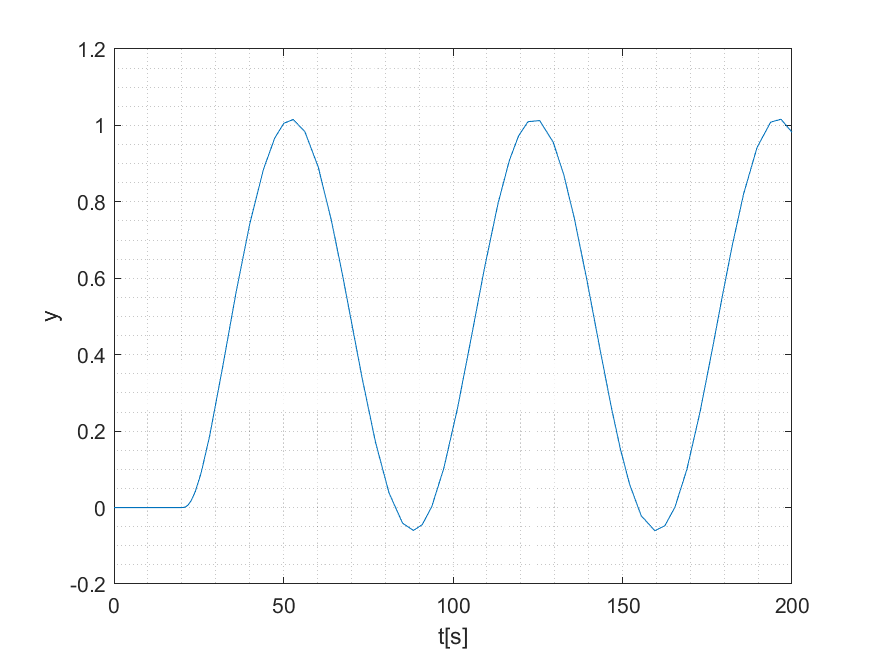
\includegraphics[width=7.5cm]{pkt4} 
\end{figure}
Na podstawie wzorów z metody Zieglera-Nicholsa obliczono: \\
$K_p=0.6*k_{kryt}=0.3894$ \\
$T_i=0.5*T_{osc}=36s$ \\
$T_d=0.125*T_{osc}=9s$ \\
Wzmocnienie dynamicznego członu różniczkującego przyjmuję $kd=6$.
\subsection{Odpowiedzi układu z zadanym sygnałem i zakłóceniem.}
\subsubsection{$y_r(t)=1(t-10), z(t)=0$}
\begin{tabular}{cc}
	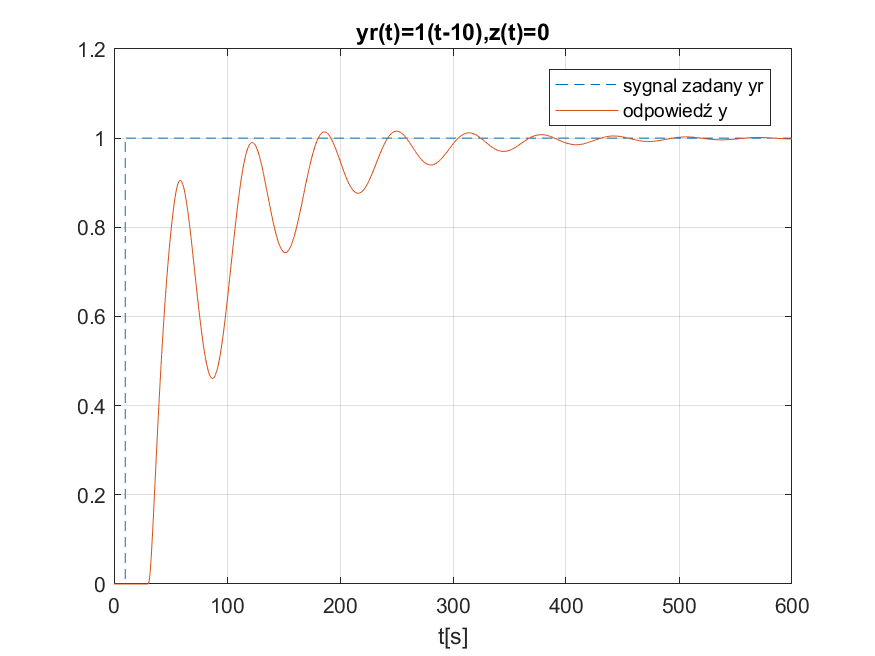
\includegraphics[width=7cm]{pkt5_1a} &	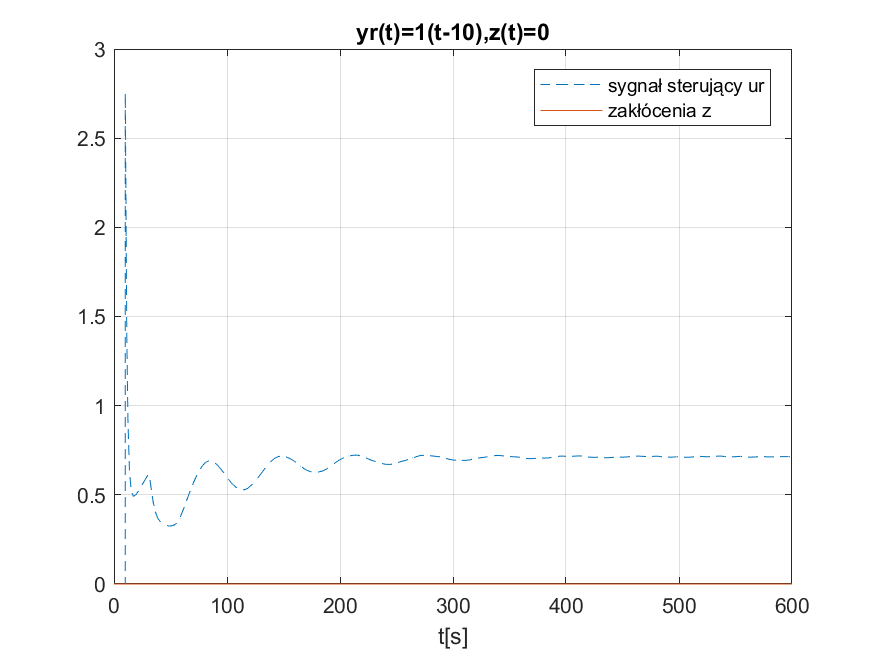
\includegraphics[width=7cm]{pkt5_1b}
\end{tabular}
\subsubsection{$y_r(t)=1(t-10), z(t)=0.2*1(t-100)$}
\begin{tabular}{cc}
	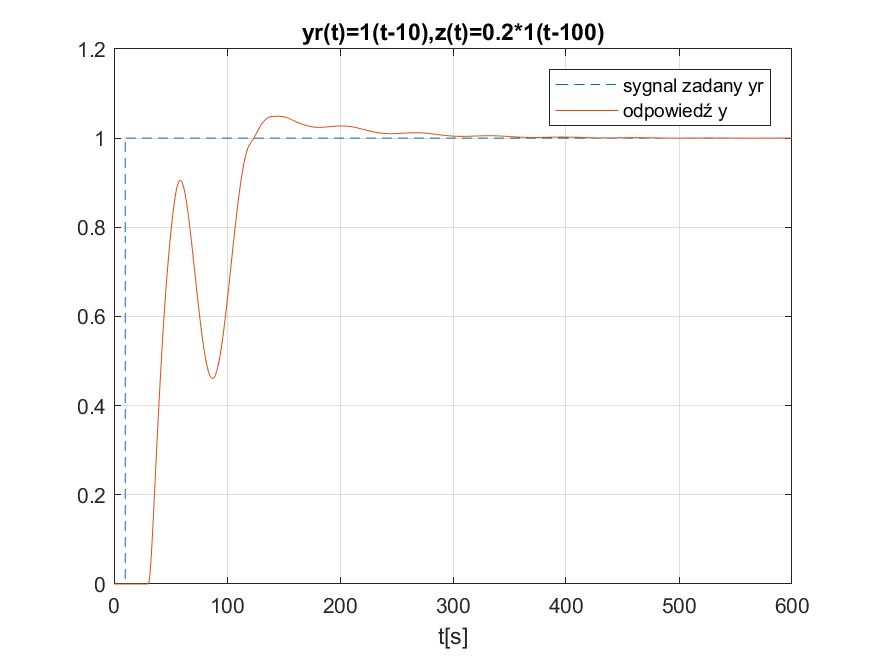
\includegraphics[width=7cm]{pkt5_2a} &	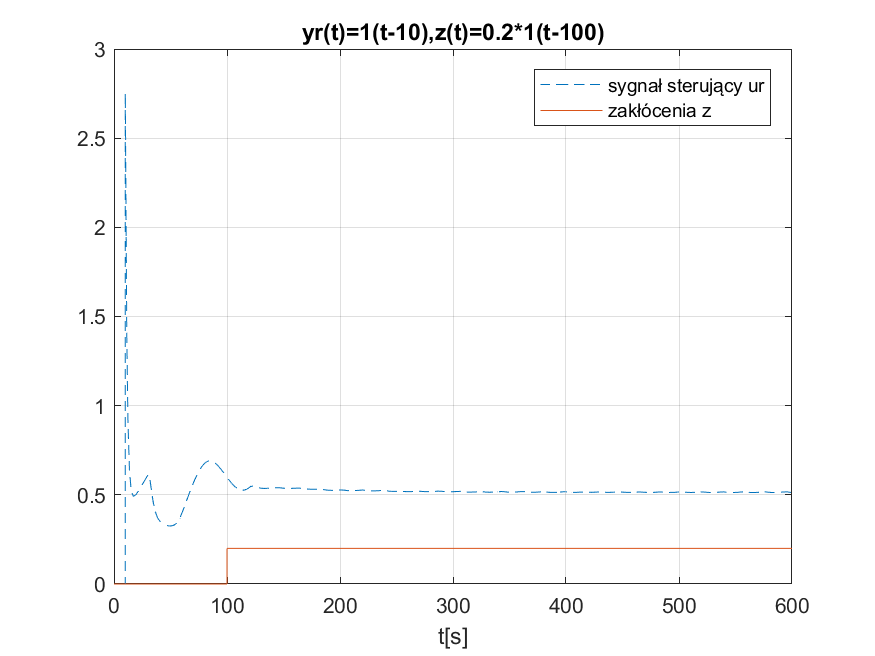
\includegraphics[width=7cm]{pkt5_2b}
\end{tabular}
\subsubsection{$y_r(t)=sin(0.01t)*1(t-10), z(t)=0$}
\begin{tabular}{cc}
	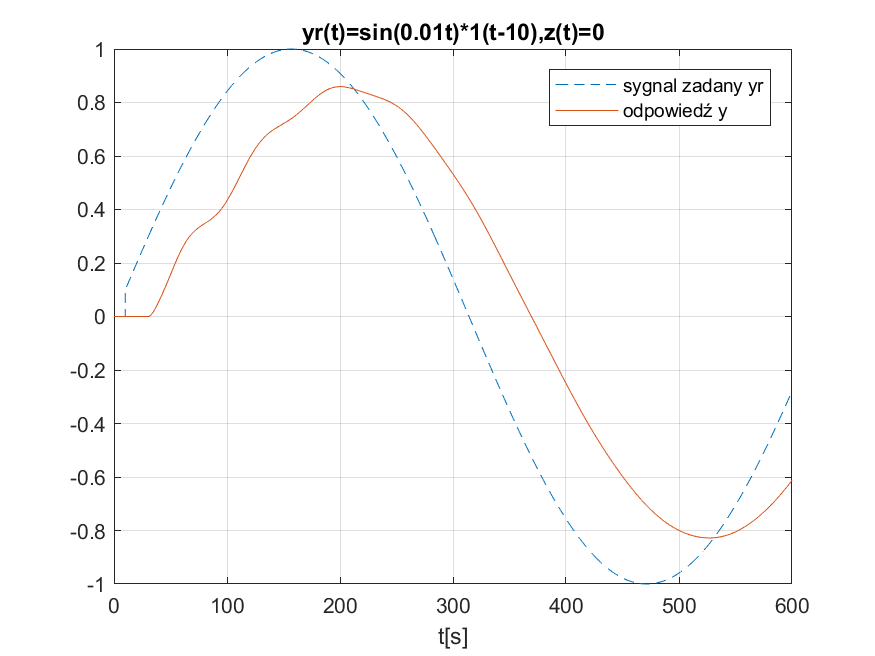
\includegraphics[width=7cm]{pkt5_3a} &	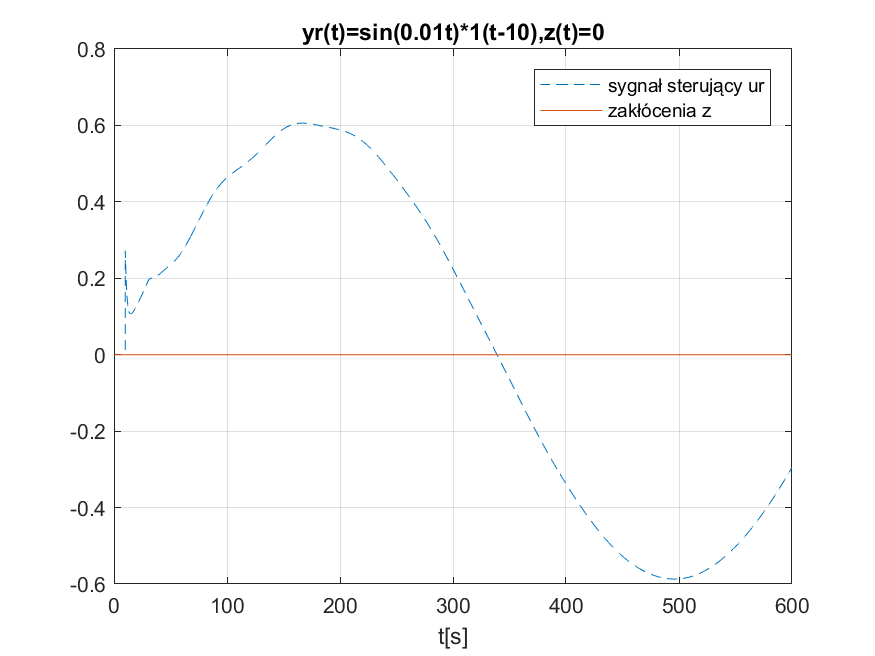
\includegraphics[width=7cm]{pkt5_3b}
\end{tabular}
\subsubsection{$y_r(t)=cos(0.05t), z(t)=0.1[1(t)-sin(0.05t)]$}
\begin{tabular}{cc}
	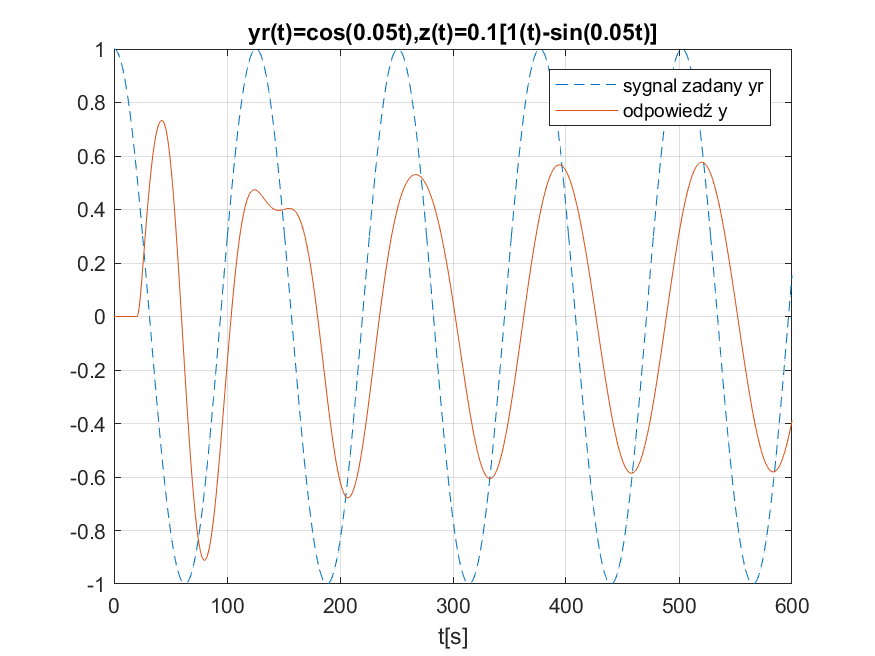
\includegraphics[width=7cm]{pkt5_4a} &	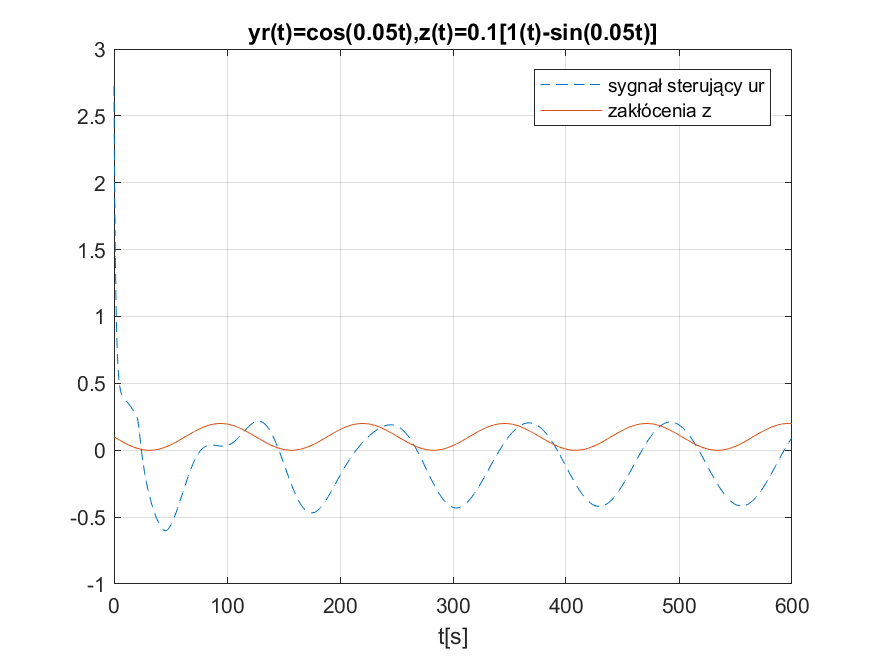
\includegraphics[width=7cm]{pkt5_4b}
\end{tabular}
\subsection{Wskaźniki jakości regulacji dla układu z pkt 5.1.}
Czas regulacji: 287.3s. Jest to czas od chwili wprowadzenia pobudzenia do chwili gdy odchyłka regulacji e osiąga wartości mieszczące się w strefie tolerancji $\pm\Delta$ ($\Delta=0.05e_m$ gdzie $e_m$ jest największą  wartością bezwzględną odchyłki e w procesie regulacji) \\
Przeregulowanie: 5.469\%. Jest to stosunek wartości drugiego uchybu przejściowego $e_2$ do wartości pierwszego uchybu przejściowego $e_{1}$  wyrażony w procentach.\\
średni błąd regulacji: 0.1101. \\
Całka kwadratu błędu regulacji: 38.2689. \\
Energia sterowania: 273.5698. \\
\section{Wnioski}

Dzięki programowi Simulink łatwo można było zasymulować model układu.
Regulator PID zapewnia dobrą jakość regulacji dla wymuszeń o charakterze skokowym. Wówczas po pewnym czasie wartość wyjściowa ustala się na poziomie sygnału zadanego. 
Dla zadanych sygnałów sinusoidalnych regulacja jest gorszej jakości. Odpowiedź nie osiągnęła odpowiedniej amplitudy oraz jest przesunięta w fazie.

\section{Kod programu}

\end{document}